\chapter{Graphene}

\section{Graphene}

Graphene is a two dimensional honeycomb lattice of carbon atoms. Each carbon atom is $sp^2$ hybridized where one $s$ orbital and two $p$ orbitals form three planar bonds with a separation angle of 120\degree. The distance between the individual carbon atoms is 1.42 Å. Due to the flexibility of the $sp^2$ bonds in the z direction, many other structures can be formed by a sheet of graphene, such as fullerenes, carbon nanotubes, and graphite. The graphene unit cell consists of only two lattice points, and the lattice vectors can be written as the following:

\begin{align*}
  a_1 = \frac{a}{2}(3,-\sqrt{3}) \; a_2 = \frac{a}{2}(3,\sqrt{3})
\end{align*}

\section{Graphene on Ir}

As a monolayer of graphene is synthesized on top of a metal surface the underlying metal and the graphene monolayer rarely has identical lattice parameters. This causes a mismatch between the two layers and these will be rotated at an angle compared to each other. A moiré superstructure appears when this surface is examined by STM, because certain areas has carbon directly above iridium, and certain areas has carbon and iridium perfectly out of phase. Below, figure \ref{moireunitcell} shows the the graphene-iridium moiré unit cell.

\begin{figure}
  \centering
  \begin{subfigure}[b]{0.3\textwidth}
       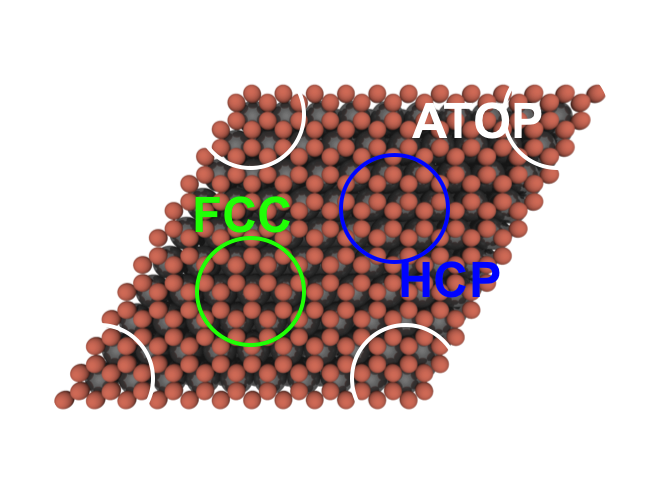
\includegraphics[width=\textwidth]{grirmoire}
       \caption{}
       \label{fig:unmarked}
   \end{subfigure}
   \begin{subfigure}[b]{0.3\textwidth}
        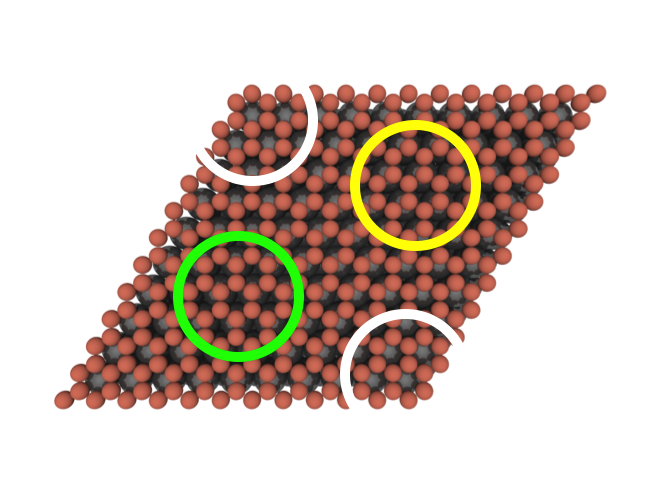
\includegraphics[width=\textwidth]{grirmoiremarked}
        \caption{}
        \label{fig:marked}
    \end{subfigure}
  \caption{Graphical interpretation of the Gr/Ir moire unit cell. \cite{Line}}
  \label{moireunitcell}
\end{figure}


\section{Hydrogenation of graphene using atomic deuterium}

The properties of graphene changes drastically with chemical functionalization of different species. The adsorption of any species is highly determined by the underlying surface, which in this study is Ir(111). The adsorption of hydrogen to the Gr/Ir surface is a highly wanted mechanism to understand, due to the special abilities arising from the functionalization of graphene by hydrogen. These effects include a bandgap opening of at least 450meV.\cite{e40134a5a1aa4cb69ba806c02cd8e327} The bandgap opens up for a large number of possibilities for the usage of functionalized graphene, where the most appealing is constructing a new type of field effect transistors. Other forms of applications of functionalized graphene is within energy storage. Due to the one atom thick monolayer it is desirable to use graphene to store hydrogen, in order to increase the hydrogen storage density.\\
As hydrogen is adsorbed to the graphene monolayer, the structural arrangement is changed. Due to the adsorbed hydrogen atom, the graphene undergoes a transition from $sp^2$ hybridization to $sp^3$ hybridization. This implies that the otherwise flat graphene sheet is twisted with the angles between the bonds in the $sp^3$ hybridization. Since every second carbon atom is turning downwards, the carbon atom constructs a bond to the underlying Ir(111) surface. This is only possible in the HCP and FCC sites of the moiré unit cell where every second carbon atom of the graphene is directly above an Iridium atom. This induce that the hydrogenation of graphene follows the moiré pattern.\cite{PhysRevB.93.115403} It is therefore expected to observe a superstructure from the hydrogenated surface with the same periodicity as the moiré pattern.\\
A graphical interpretation of the hydrogenation of graphene on Ir(111) is shown in figure \ref{hydrogenation:all}, which is made by Line Kyhl. Here it is seen that clusters of hydrogen bind to the carbon atoms in the FCC and HCP sites. Figure \ref{hydrogenationside} demonstrates how every other carbon atom binds to the Ir(111) surface and every other binds to a hydrogen atom. Furthermore dimers of hydrogen is seen bind to the surface at the ATOP sites. In these regions the distance to the surface Iridium surface is

\begin{figure}
  \centering
  \begin{subfigure}[b]{0.3\textwidth}
       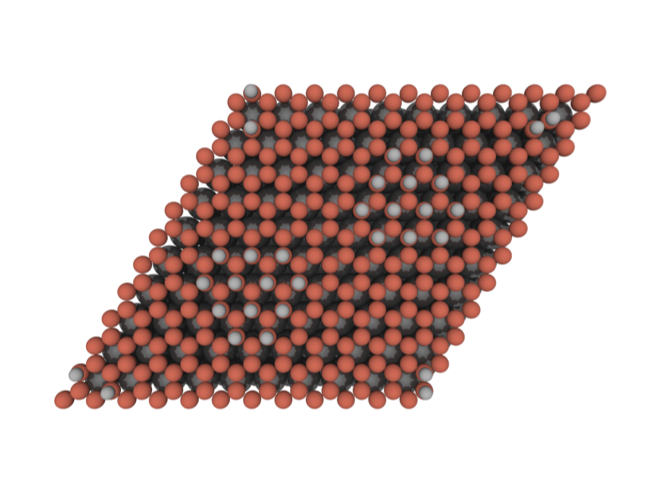
\includegraphics[width=\textwidth]{atomichydrogenation}
       \caption{}
       \label{hydrogenation}
   \end{subfigure}
   \begin{subfigure}[b]{0.3\textwidth}
        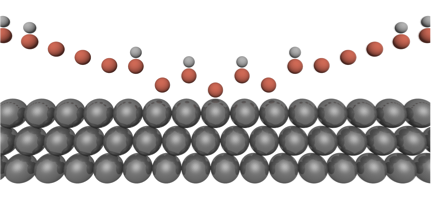
\includegraphics[width=\textwidth]{atomichydrogenationside}
        \caption{}
        \label{hydrogenationside}
    \end{subfigure}
  \caption{Graphical interpretation of the }
  \label{hydrogenation:all}
\end{figure}



\section{Hydrogenation of graphene using vibrationally excited deuterium}

\begin{align}
  \phi (H) = 2 s_m P_a \phi (H_2)
\end{align}

\begin{align}
  P_a = \frac{1}{4} [\{(K_p/\gamma p)(K_p / \gamma p + 8)\}^{\frac{1}{2}} -K_p/\gamma p]
\end{align}


\begin{figure}
  \centering
  \begin{subfigure}[b]{0.3\textwidth}
       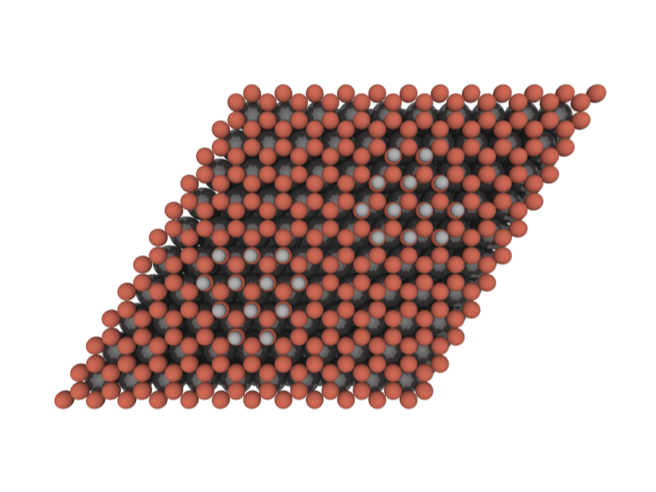
\includegraphics[width=\textwidth]{molecularhydrogenation}
       \caption{}
       \label{molhydrogenation}
   \end{subfigure}
   \begin{subfigure}[b]{0.3\textwidth}
        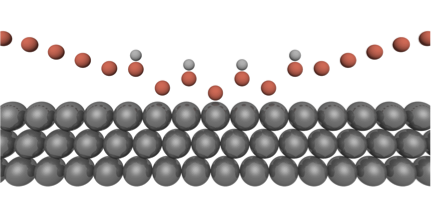
\includegraphics[width=\textwidth]{molecularhydrogenationside}
        \caption{}
        \label{molhydrogenationside}
    \end{subfigure}
  \caption{Graphical interpretation of the }
  \label{molhydrogenation:all}
\end{figure}
